\documentclass[dvipdfmx]{jarticle}
\pagestyle{empty}
\usepackage{tikz}
\usetikzlibrary{shapes,calc}
\begin{document}
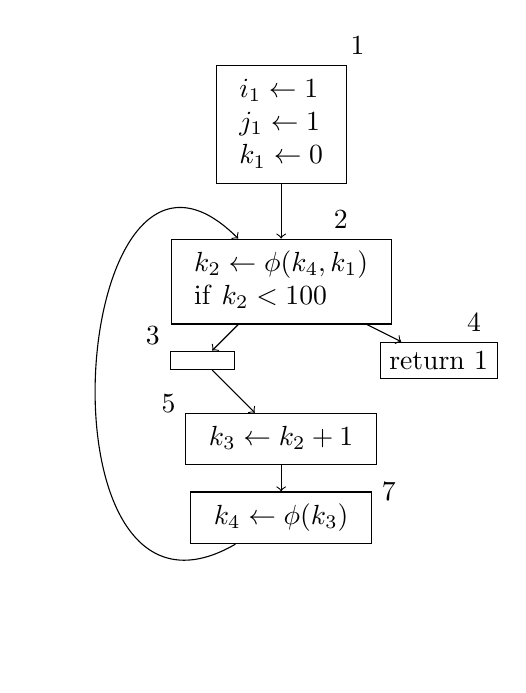
\begin{tikzpicture}
  \node[draw,label={45:$1$}] (B1) at (0,0) {
    $\begin{array}{l}
      i_1\leftarrow 1\\
      j_1\leftarrow 1\\
      k_1\leftarrow 0
  \end{array}$};
  \node[draw,label={45:$2$}] (B2) at (0,-2) {
    $\begin{array}{l}
%      j_2\leftarrow\phi(j_4,j_1)\\
      k_2\leftarrow\phi(k_4,k_1)\\
      \mathrm{if}\ k_2<100
    \end{array}$};
  \node[draw,label={170:$3$}] (B3) at (-1,-3) {
    \mbox{\ \ \ \ \ }
  };
  \node[draw,label={45:$4$}] (B4) at (2,-3) {
    $\mathrm{return}\ 1$
  };
  \node[draw,label={170:$5$}] (B5) at (0,-4) {
    $\begin{array}{l}
%      j_3\leftarrow i_1\\
      k_3\leftarrow k_2+1
    \end{array}$
  };
  % \node[draw,label={15:$6$}] (B6) at (1,-5.5) {
  %   $\begin{array}{l}
  %     j_5\leftarrow k_2\\
  %     k_5\leftarrow k_2+2
  %   \end{array}$
  % };
  \node[draw,label={5:$7$}] (B7) at (0,-5) {
    $\begin{array}{l}
%      j_4\leftarrow\phi(j_3,j_5)\\
      k_4\leftarrow\phi(k_3)
    \end{array}$
  };
  \path[->] (B1) edge (B2) (B2) edge (B3) (B2) edge (B4);
  \path[->] (B3) edge (B5);
  \path[->] (B5) edge (B7);
  \path[->,out=210,in=135,looseness=2] (B7) edge (B2);
\end{tikzpicture}
\end{document}